% Options for packages loaded elsewhere
\PassOptionsToPackage{unicode}{hyperref}
\PassOptionsToPackage{hyphens}{url}
%
\documentclass[
]{book}
\usepackage{amsmath,amssymb}
\usepackage{lmodern}
\usepackage{iftex}
\ifPDFTeX
  \usepackage[T1]{fontenc}
  \usepackage[utf8]{inputenc}
  \usepackage{textcomp} % provide euro and other symbols
\else % if luatex or xetex
  \usepackage{unicode-math}
  \defaultfontfeatures{Scale=MatchLowercase}
  \defaultfontfeatures[\rmfamily]{Ligatures=TeX,Scale=1}
\fi
% Use upquote if available, for straight quotes in verbatim environments
\IfFileExists{upquote.sty}{\usepackage{upquote}}{}
\IfFileExists{microtype.sty}{% use microtype if available
  \usepackage[]{microtype}
  \UseMicrotypeSet[protrusion]{basicmath} % disable protrusion for tt fonts
}{}
\makeatletter
\@ifundefined{KOMAClassName}{% if non-KOMA class
  \IfFileExists{parskip.sty}{%
    \usepackage{parskip}
  }{% else
    \setlength{\parindent}{0pt}
    \setlength{\parskip}{6pt plus 2pt minus 1pt}}
}{% if KOMA class
  \KOMAoptions{parskip=half}}
\makeatother
\usepackage{xcolor}
\IfFileExists{xurl.sty}{\usepackage{xurl}}{} % add URL line breaks if available
\IfFileExists{bookmark.sty}{\usepackage{bookmark}}{\usepackage{hyperref}}
\hypersetup{
  pdftitle={Computational Biology for All!},
  pdfauthor={Nathan L. BRouwer},
  hidelinks,
  pdfcreator={LaTeX via pandoc}}
\urlstyle{same} % disable monospaced font for URLs
\usepackage{color}
\usepackage{fancyvrb}
\newcommand{\VerbBar}{|}
\newcommand{\VERB}{\Verb[commandchars=\\\{\}]}
\DefineVerbatimEnvironment{Highlighting}{Verbatim}{commandchars=\\\{\}}
% Add ',fontsize=\small' for more characters per line
\usepackage{framed}
\definecolor{shadecolor}{RGB}{248,248,248}
\newenvironment{Shaded}{\begin{snugshade}}{\end{snugshade}}
\newcommand{\AlertTok}[1]{\textcolor[rgb]{0.94,0.16,0.16}{#1}}
\newcommand{\AnnotationTok}[1]{\textcolor[rgb]{0.56,0.35,0.01}{\textbf{\textit{#1}}}}
\newcommand{\AttributeTok}[1]{\textcolor[rgb]{0.77,0.63,0.00}{#1}}
\newcommand{\BaseNTok}[1]{\textcolor[rgb]{0.00,0.00,0.81}{#1}}
\newcommand{\BuiltInTok}[1]{#1}
\newcommand{\CharTok}[1]{\textcolor[rgb]{0.31,0.60,0.02}{#1}}
\newcommand{\CommentTok}[1]{\textcolor[rgb]{0.56,0.35,0.01}{\textit{#1}}}
\newcommand{\CommentVarTok}[1]{\textcolor[rgb]{0.56,0.35,0.01}{\textbf{\textit{#1}}}}
\newcommand{\ConstantTok}[1]{\textcolor[rgb]{0.00,0.00,0.00}{#1}}
\newcommand{\ControlFlowTok}[1]{\textcolor[rgb]{0.13,0.29,0.53}{\textbf{#1}}}
\newcommand{\DataTypeTok}[1]{\textcolor[rgb]{0.13,0.29,0.53}{#1}}
\newcommand{\DecValTok}[1]{\textcolor[rgb]{0.00,0.00,0.81}{#1}}
\newcommand{\DocumentationTok}[1]{\textcolor[rgb]{0.56,0.35,0.01}{\textbf{\textit{#1}}}}
\newcommand{\ErrorTok}[1]{\textcolor[rgb]{0.64,0.00,0.00}{\textbf{#1}}}
\newcommand{\ExtensionTok}[1]{#1}
\newcommand{\FloatTok}[1]{\textcolor[rgb]{0.00,0.00,0.81}{#1}}
\newcommand{\FunctionTok}[1]{\textcolor[rgb]{0.00,0.00,0.00}{#1}}
\newcommand{\ImportTok}[1]{#1}
\newcommand{\InformationTok}[1]{\textcolor[rgb]{0.56,0.35,0.01}{\textbf{\textit{#1}}}}
\newcommand{\KeywordTok}[1]{\textcolor[rgb]{0.13,0.29,0.53}{\textbf{#1}}}
\newcommand{\NormalTok}[1]{#1}
\newcommand{\OperatorTok}[1]{\textcolor[rgb]{0.81,0.36,0.00}{\textbf{#1}}}
\newcommand{\OtherTok}[1]{\textcolor[rgb]{0.56,0.35,0.01}{#1}}
\newcommand{\PreprocessorTok}[1]{\textcolor[rgb]{0.56,0.35,0.01}{\textit{#1}}}
\newcommand{\RegionMarkerTok}[1]{#1}
\newcommand{\SpecialCharTok}[1]{\textcolor[rgb]{0.00,0.00,0.00}{#1}}
\newcommand{\SpecialStringTok}[1]{\textcolor[rgb]{0.31,0.60,0.02}{#1}}
\newcommand{\StringTok}[1]{\textcolor[rgb]{0.31,0.60,0.02}{#1}}
\newcommand{\VariableTok}[1]{\textcolor[rgb]{0.00,0.00,0.00}{#1}}
\newcommand{\VerbatimStringTok}[1]{\textcolor[rgb]{0.31,0.60,0.02}{#1}}
\newcommand{\WarningTok}[1]{\textcolor[rgb]{0.56,0.35,0.01}{\textbf{\textit{#1}}}}
\usepackage{longtable,booktabs,array}
\usepackage{calc} % for calculating minipage widths
% Correct order of tables after \paragraph or \subparagraph
\usepackage{etoolbox}
\makeatletter
\patchcmd\longtable{\par}{\if@noskipsec\mbox{}\fi\par}{}{}
\makeatother
% Allow footnotes in longtable head/foot
\IfFileExists{footnotehyper.sty}{\usepackage{footnotehyper}}{\usepackage{footnote}}
\makesavenoteenv{longtable}
\usepackage{graphicx}
\makeatletter
\def\maxwidth{\ifdim\Gin@nat@width>\linewidth\linewidth\else\Gin@nat@width\fi}
\def\maxheight{\ifdim\Gin@nat@height>\textheight\textheight\else\Gin@nat@height\fi}
\makeatother
% Scale images if necessary, so that they will not overflow the page
% margins by default, and it is still possible to overwrite the defaults
% using explicit options in \includegraphics[width, height, ...]{}
\setkeys{Gin}{width=\maxwidth,height=\maxheight,keepaspectratio}
% Set default figure placement to htbp
\makeatletter
\def\fps@figure{htbp}
\makeatother
\setlength{\emergencystretch}{3em} % prevent overfull lines
\providecommand{\tightlist}{%
  \setlength{\itemsep}{0pt}\setlength{\parskip}{0pt}}
\setcounter{secnumdepth}{5}
\usepackage{booktabs}
\ifLuaTeX
  \usepackage{selnolig}  % disable illegal ligatures
\fi
\usepackage[]{natbib}
\bibliographystyle{apalike}

\title{Computational Biology for All!}
\author{Nathan L. BRouwer}
\date{2021-08-15}

\begin{document}
\maketitle

{
\setcounter{tocdepth}{1}
\tableofcontents
}
\hypertarget{preface}{%
\chapter*{Preface}\label{preface}}
\addcontentsline{toc}{chapter}{Preface}

\hypertarget{part-introduction}{%
\part{Introduction}\label{part-introduction}}

\hypertarget{predface}{%
\subsection*{Predface}\label{predface}}
\addcontentsline{toc}{subsection}{Predface}

In Book 1 I'll introduce why the role of computers in biology is important and lay out the scope of this book. I'll also walk through the basic steps of getting R and RStudio up and running on your computer, walk through a basic R session, and discuss the various ways we'll interact with R using \textbf{code} and \textbf{script files}. I'll also introduce \textbf{rmarkdown}, a way of integrating the R code of scripts with basic capabilities of word processing and web development. Scripts organized in rmarkdown are a handy way to organize and \textbf{annotate code}, store and disseminate your work, and structure your analyses and data presentations so that the computations behind them are fully \textbf{reproducible}.

\hypertarget{intro}{%
\chapter{Welcome to computational biology for all!}\label{intro}}

Welcome to \emph{Computational Biology for All!}.

This book will introduce you to key concepts of computational biology using the software R. It covers such topics as statistics, data science, bioinformatics, building phylogenetic trees, and building computer models of biological processes.

I will make only two assumptions in this book:

\begin{enumerate}
\def\labelenumi{\arabic{enumi}.}
\tightlist
\item
  You are interested in biology and need a computer to answer a question
\item
  You've had some college-level biology or are willing to read some basic background information in the book, the appendices or the internet.
\end{enumerate}

That's it. If you've forgotten how many amino acids are specified by the genetic code (or never learned; its 20), have never run computer code, or aren't sure what ``computational biology'' is no worries. We'll work through everything step by step, review often, and link to additional resources.

\hypertarget{r-and-rstudio---your-new-best-friends}{%
\section{R and RStudio - your new best friends!}\label{r-and-rstudio---your-new-best-friends}}

\textbf{R} is one of the major computer languages used by scientists. ``R'' refers both to the computer language itself, and to the base software which runs the computer code for us. Most people write and run their code in a special program that acts like a word processor for coding; these goes by the fancy name \textbf{Integrated Development Environments} or \textbf{IDEs}. In this book we'll use the popular IDE software called \textbf{RStudio}.

You should get access to the software combination of the software \textbf{R} and \textbf{RStudio(())} either on the cloud via an account with (\textbf{RStudio Cloud}){[}\url{https://rstudio.cloud/}{]} or on your own hard drive. (Some institutions may have their own special implementation of R and RStudio; ask your tech support about this.)

If your are brand-new to using R the easiest way to get started is using RStudio Cloud. Getting R and RStudio set up on your own computer isn't (usually) difficult, but RStudio Cloud even easier. For information on R, RStudio, and RStudio Cloud see the Appendices. There are also many videos on the internet walking you through these topics.

If I've already lost you a bit with any of this information don't worry - we'll cover more details in the following chapters, and the Appendices cover how to get start with R, RStudio, and RStudio step-by-step.

\hypertarget{how-to-use-this-book---be-an-active-learner}{%
\section{How to use this book - be an active learner!}\label{how-to-use-this-book---be-an-active-learner}}

While you can read this as a regular book, it is meant to be an \textbf{active learning text}. That means you'll get much more out of it if you are working through all the code step by step. There are two ways to do this:

\begin{enumerate}
\def\labelenumi{\arabic{enumi}.}
\tightlist
\item
  Read the book like a book (printed, PDF, website) and type the code in RStudio.
\item
  Download the associated \textbf{Active Learning Notebooks} and work through them in RStudio.
\end{enumerate}

The \textbf{Active Learning Notebooks} contain \textbf{ALL} of the text and code, and is the recommended way to experience the book.

\hypertarget{biological-scope-of-this-book}{%
\section{Biological scope of this book}\label{biological-scope-of-this-book}}

``Computational Biology'' means different things to different people, and I'll discuss how it can be defined in a later chapter. In general, though, I'll apply a very broad definition and touch upon all aspects of biology, from biochemistry to ecology. My starting point will generally by the topics classically associated with computational biology: bioinformatics, genomics, and building phylogenetic trees. Moreover, when I cover other topics like population dynamics or community ecology I'll often use molecular-biology related examples, such as population growth of transposons in our genomes and community diversity of bacteria in our guts (the so-called gut microbiome, which is studied using molecular sequencing technologies). If you're primary interest is in ecology everything in this book will be applicable at the very least in terms of the techniques, and hopefully it will help everyone expand their idea of how ecological concepts can be applied.

\hypertarget{what-is-computational-biology}{%
\chapter{What is Computational Biology?}\label{what-is-computational-biology}}

This is mostly notes.

\hypertarget{notes}{%
\section{Notes}\label{notes}}

\hypertarget{nih-definition}{%
\subsection{NIH definition}\label{nih-definition}}

See file NIH\_def\_bioinfo\_2000.rmd for full text of the NIH document

\textbf{NOTES}:

\begin{itemize}
\tightlist
\item
  bioinformatics relevant to all life sciences (not just biology)
\item
  Bioinf/comp bio both ``rooted'' in life science, comp sci, info sci and technologies
\item
  Bioinformatics: application focused, access / understanding from data
\item
  Comp bio: theory/discovery approaches
\end{itemize}

\begin{quote}
\emph{Bioinformatics:} Research, development, or application of computational tools and approaches for expanding the use of biological, medical, behavioral or health data, including those to acquire, store, organize, archive, analyze, or visualize such data.
\end{quote}

\begin{quote}
\emph{Computational Biology:} The development and application of data-analytical and
theoretical methods, mathematical modeling and computational simulation techniques
to the study of biological, behavioral, and social systems
\end{quote}

\hypertarget{luscombe-et-al-2001}{%
\section{Luscombe et al 2001}\label{luscombe-et-al-2001}}

N.M. Luscombe, D. Greenbaum, M. Gerstein. Bioinformatics definition committee. 2001. What is Bioinformatics? A Proposed Definition and Overview of the Field \url{https://www.thieme-connect.com/products/ejournals/abstract/10.1055/s-0038-1634431}

\begin{quote}
``Our definition is as follows: Bioinformatics is conceptualizing biology in terms of macromolecules (in the sense of physical-chemistry) and then applying ``informatics'' techniques (derived from disciplines such as applied maths, computer science, and statistics) to understand and organize the information associated with these molecules, on a large-scale.'' Luscombe et al 2000
\end{quote}

\begin{quote}
``Analyses in bioinformatics predominantly focus on three types of large datasets available in molecular biology: macromolecular structures, genome sequences, and the results of functional genomics experiments (eg expression data). Additional information includes the text of scientific papers and ``relationship data'' from metabolic pathways, taxonomy trees, and protein-protein interaction networks.'' Luscombe et al 2000
\end{quote}

\hypertarget{taprich-et-al-20121}{%
\section{Taprich et al 20121}\label{taprich-et-al-20121}}

Taprich et al.~2021. An instructional definition and assessment rubric for bioinformatics instruction. \url{https://iubmb.onlinelibrary.wiley.com/doi/full/10.1002/bmb.21361}

\begin{quote}
``An interdisciplinary field that is concerned with the development and application of algorithms that analyze biological data to investigate the structure and function of biological polymers and their relationships to living systems.''
\end{quote}

\hypertarget{smith-2015-frontiers-in-genetics}{%
\section{Smith 2015 Frontiers in Genetics}\label{smith-2015-frontiers-in-genetics}}

Smith. 2015. Broadening the definition of a bioinformatician. Frontiers in Genetics
\url{https://www.frontiersin.org/articles/10.3389/fgene.2015.00258/full}

\begin{quote}
``On a given day, I spend much of my research time staring at nucleotide sequences on a computer screen and theorizing about the evolution of genomes; thus, I feel comfortable calling myself a bioinformatician, or at the very least a scientist who primarily uses bioinformatics for his research. If asked, most of my colleagues, mentors, and students would also define me as a bioinformatician. But there is one small catch: I don't know how to program computer software or curate databases, and I am even quite pathetic at writing UNIX commands, which according to some precludes me from having the title of bioinformatician.'' Smith (2015)
\end{quote}

\begin{quote}
``I imagine that many of the scientists reading this essay will consider me an imposter, an amateur who points, clicks, and stumbles his way through the complicated landscape of bioinformatics. \ldots{} I believe that as a research community we need to broaden our definition of what it means to be a bioinformatician, not restricting it to only those who develop software or design and maintain data resources. \ldots{} {[}T{]}he term bioinformatician should encompass the countless and ever growing number of scientists who use computers and bioinformatics programs to address fundamental questions in biology.'' Smith (2015)
\end{quote}

\hypertarget{good-readings-references}{%
\section{Good readings / references}\label{good-readings-references}}

Koonin, EV. 20xx. Primer: Computational genomics. Current Biology - Magazine. R155-158\ldots{}

\hypertarget{potential-references}{%
\section{Potential references}\label{potential-references}}

\url{https://asistdl.onlinelibrary.wiley.com/doi/full/10.1002/asi.20133?casa_token=iDFXKee8e1gAAAAA\%3AD7vtxphVMi2MHDEIvWi7Y3twQcKUvdI5Co3pF11-OgoTdk1dEHe8H5XKv67mnz1uyGyFRoMeqrbeY_Q}

\url{https://www.geneticsmr.com/sites/default/files/articles/year2017/vol16-1/pdf/gmr-16-01-gmr.16019645_0.pdf}

\url{https://ieeexplore.ieee.org/abstract/document/1678036?casa_token=H9KSAnKN-XIAAAAA:R_uzPueqLDOCWccNZgdRkaRxpOo3J2RSMpVG7ZLAebTVp0-tqGl0TKQderfudEOS2efgl9oWVw}
\url{https://dl.acm.org/doi/abs/10.1145/1031120.1031122?casa_token=YBJzo0bknd8AAAAA:tzp2T3uGqb1MXRPtSccpKXAyKqtmTORa6B_yWGA9dQ9Pj4UElgeH8LK0hVJ_2PaAF51I3oqY8N-EkA}

\hypertarget{original-info-from-eco-data-science-project}{%
\section{Original info, from Eco Data Science project}\label{original-info-from-eco-data-science-project}}

\textbf{{[}NOTE: This section is currently under development. The paper by Touchon \& McCoy (2016) and its references lay out many of the reasons for the statistical focus of this book and relates to all biology, not just ecology.{]}}

\begin{quote}
``Ecological questions and data are becoming increasingly complex and as a result we are seeing the development and proliferation of sophisticated statistical approaches in the ecological literature. \ldots{} It is no longer sufficient to only ask `whether' or `which' experimental manipulations significantly deviate from null expectations. Instead, we are moving toward parameter estimation and asking \textbf{`how much'} and in \textbf{`what direction'} ecological processes are affected by different mechanisms'' (\href{https://esajournals.onlinelibrary.wiley.com/doi/abs/10.1002/ecs2.1394}{Touchon \& McCoy 2016, Ecosphere}, emphsis mine)
\end{quote}

\begin{quote}
``Spreadsheets are often used as the basis of data collection and education; but this is potentially problematic since spreadsheets typically do not promote good data management practices\ldots. The features of spreadsheets that make them desirable for the average researcher, such as extensibility, use of formatting for organization, embedding charts, make them undesirable for preparing data for long‐term archiving and reuse.''(\href{https://esajournals.onlinelibrary.wiley.com/doi/abs/10.1890/ES12-00139.1}{Strasser \& Hampton 2012 Ecosphere})
\end{quote}

\hypertarget{what-is-data-science}{%
\section{What is data science?}\label{what-is-data-science}}

\begin{quote}
Data analysis include ``procedures for analyzing data, techniques for interpreting the results\ldots, ways of planning the gathering of data to make its analysis easier, more precise or more accurate, and all the machinery and results of (mathematical) statistics which apply to analyzing data.'' John Tukey, ``The future of data analysis'', Annals of Mathematical Statistics, 1962.
\end{quote}

\begin{itemize}
\tightlist
\item
  People argue about what data science is
\item
  What Tukey calls ``data analysis'' is now termed ``data science'' by many.\\
\item
  Some define data science as closely allied with computer science and want its use most closely associated with things like ``big data'', data mining, machine learning, and artificial intelligence.
\item
  Others, such as RStudio's Hadley Whickham (creator of ggplot2, dplyr, and most of the infrasture of the tidyverse of R package) define it more broadly to involve all aspects of the life cycle of data.
\item
  (Wickham also defines a data scientists as ``A data scientist is a statistician who is wearing a bow tie'' \url{https://twitter.com/hadleywickham/status/906146116412039169?lang=en})
\end{itemize}

\hypertarget{refereces}{%
\section{Refereces}\label{refereces}}

Strasser \& Hampton 2012. The fractured lab notebook: undergraduates and ecological data management training in the United States. EcoSphere. \url{https://esajournals.onlinelibrary.wiley.com/doi/abs/10.1890/ES12-00139.1}

Touchon \& McCoy 2017. The mismatch between current statistical practice and doctoral training in ecology. EcoSphere. \url{https://esajournals.onlinelibrary.wiley.com/doi/abs/10.1002/ecs2.1394}

Tukey. 1962. The future of data analysis. Annals of Mathematical Statistics. \url{https://www.jstor.org/stable/2237638}

\hypertarget{bibliography}{%
\section{Bibliography}\label{bibliography}}

Relevant papers cited by Touchon \& McOy 2017.

Barraquand, F., T. H. G. Ezard, P. S. Jørgensen, N. Zimmerman, S. Chamberlain, R. Salguero‐Gómez, T. J. Curran, and T. Poisot. 2014. Lack of quantitative training among early‐career ecologists: a survey of the problem and potential solutions. PeerJ 2:e285.

Butcher, J. A., J. E. Groce, C. M. Lituma, M. C. Cocimano, Y. Sánchez‐Johnson, A. J. Campomizzi, T. L. Pope, K. S. Reyna, and A. C. S. Knipps. 2007. Persistent controversy in statistical approaches in wildlife sciences: a perspective of students. Journal of Wildlife Management 71:2142--2144

Ellison, A. M., and B. Dennis. 2009. Paths to statistical fluency for ecologists. Frontiers in Ecology and the Environment 8:362--370.

Germano, J. D. 2000. Ecology, statistics, and the art of misdiagnosis: the need for a paradigm shift. Environmental Reviews 7:167--190.

Quinn, J. F., and A. E. Dunham. 1983. On hypothesis testing in ecology and evolution. American Naturalist 122:602--617.

\hypertarget{how-will-this-book-teach-computational-biology}{%
\chapter{How will this book teach computational biology?}\label{how-will-this-book-teach-computational-biology}}

\begin{quote}
``The rise of computer programming, computational power, and modern statistical approaches may\ldots{}'' allow ``\ldots scientists to ask new questions and to extract more information from data than ever before.'' (\href{https://esajournals.onlinelibrary.wiley.com/doi/abs/10.1002/ecs2.1394}{Touchon \& McCoy 2016, Ecosphere})
\end{quote}

\hypertarget{what-youll-learn}{%
\section{What you'll learn}\label{what-youll-learn}}

\hypertarget{general-skills-that-youll-learn}{%
\subsection{General skills that you'll learn}\label{general-skills-that-youll-learn}}

\begin{itemize}
\tightlist
\item
  \textbf{Statistical computing} using R, RStudio, and rmarkdown
\item
  \textbf{Data analysis}, from t-tests to mixed models in R
\item
  \textbf{Data visualization}, with an emphasis on ggplot2
\item
  \textbf{Data science}, from data management best practices to data cleaning with dplyr
\item
  \textbf{Computational reproducibility}, from formatting scripts to using rmarkdown to write reproducible reports
\end{itemize}

\hypertarget{computational-biology-skills-youll-learn}{%
\subsection{Computational biology skills you'll learn}\label{computational-biology-skills-youll-learn}}

\begin{itemize}
\tightlist
\item
  Working with sequence data
\item
  alignments
\item
  Phylogenetics
\item
  \ldots{}
\end{itemize}

\hypertarget{teaching-approach}{%
\section{Teaching approach}\label{teaching-approach}}

\begin{itemize}
\tightlist
\item
  Always explore and visualize data
\item
  Step-by-step instructions
\item
  Frequently refreshing and review
\item
  Comprehensive and self-contained
\item
  Worked example
\item
  ``Modify this code'' tasks
\item
  Code completion tasks (key steps missing)
\item
  Broken code tasks (fix non-functional code)
\item
  Links to Jupyter notebooks (not yet implemented)
\item
  ``Active Learning Notebooks'' - all content and code in .Rmd format
\end{itemize}

\hypertarget{requirements}{%
\section{Requirements}\label{requirements}}

\begin{itemize}
\tightlist
\item
  R
\item
  RStudio
\item
  External packages loaded via RStudio
\end{itemize}

\hypertarget{whats-not-in-this-book-course}{%
\section{What's not in this book / course}\label{whats-not-in-this-book-course}}

\hypertarget{what-is-r-and-why-use-it}{%
\chapter{What is R and why use it?}\label{what-is-r-and-why-use-it}}

{[}these notes are from a lecture and have not been re-written much yet{]}

R is a powerful piece of software used for data science and data analysis. In this chapter I will briefly introduce the advantages of using R, why you might want to learn it, and also indicate some alternatives and adjuncts you could consider.

\hypertarget{how-do-we-typically-use-software-in-science}{%
\section{How do we typically use software in science?}\label{how-do-we-typically-use-software-in-science}}

Most scientists rely on both general and specialized pieces of software for various parts of their work. For data entry they likely use spreadsheet software Excel, though increasingly Google Sheets. For data analysis they might use one of many options, such as \href{https://www.graphpad.com/}{GraphPad Prism}, Minitab, SAS, SPSS, or STATA. For making plots, many people will export their export their results back to Excel, while others use specialized software like SigmaPlot. Many scientists also use specialized programs; in ecology many researchers do GIS in ArcGIS or QGIS, mark-recapture analysis in Program MARK or Distance, use RAMAS or Vortex for population viability analysis, or build custom mathematical programs in MatLab or Python. If they do \href{https://en.wikipedia.org/wiki/Multivariate_statistics}{multivariate statistics} like {[}ordination{]}(\url{https://en.wikipedia.org/wiki/Ordination_(statistics)} the may use a specialized stats program like PC-ORD.

Since software can be expensive, some scientists will rely on Excel for all of their work. Excel can do many things, but it can't do everything all the specialized types of software can do. Moreover, its very limited in the range of statistics it can do and graphs it can make.

\hypertarget{what-does-r-do}{%
\section{What does R do?}\label{what-does-r-do}}

R is amazing because it has been explicitly developed to do several things very well, particularly statistics, math, making great-looking figures, and writing computer programs to automate these tasks. Additionally, R has been extended by developers to be able to be a powerful tool for data cleaning and organization, to be used as a GIS, and as an integrated word processor and website make for publishing work.

\hypertarget{why-use-r}{%
\section{Why use R}\label{why-use-r}}

In addition to is many capabilities, R has the advantage this it is

\begin{itemize}
\tightlist
\item
  free anyone, always
\item
  used by statisticians to develop new statistical techniques, so new techniques often come out 1st in R
\item
  used by almost all ecological statisticians to develop new techniques (mark recapture, distance sampling)
\end{itemize}

\hypertarget{who-uses-it}{%
\section{Who uses it?}\label{who-uses-it}}

R continues to increase in popularity. Among data scientists it is second only to Python. Among academics it has eclipsed SAS in many fields. It is also used by analyses in many large companies, such Facebook, and by journalists looking for stories in or reporting on large volumes of data

see \url{http://blog.revolutionanalytics.com/2014/05/companies-using-r-in-2014.html} for further discussion.

\hypertarget{r-and-computational-reproducibility}{%
\section{R and computational reproducibility}\label{r-and-computational-reproducibility}}

One factor potentially contributing to R's popularity, or at least a major bonus for using it, is ease of use for making analyses reproducible. All commands in R are typed out and the best way to do this is in a static \textbf{script file} from which you send commands to R to execute. This creates a record of your analyses. This feature is shared by other programs such as SAS and Stats, and other programming languages such as Matlab and Python. The advantage of R is that the script files are simply plain text files which anyone can open and - if they've downloaded R, which is free - they can run. Developers have also created numerous tools for creating \textbf{reproducible analysis workflows} and which allow R to be used in all data-related aspects of a project, from \textbf{data cleaning} to \textbf{formatting journal submissions}. What this means is that without become an expert programmer you can set up your work so that you can re-run all of your data cleaning, analyses, and graph building with a single command in R. This makes what you've done auditable, transparent, and easy to re-use for future work.

\hypertarget{alternatives-to-r}{%
\section{Alternatives to R}\label{alternatives-to-r}}

R has many advantages, but it has one critical issue: the learning curve. R is a command-line driven analysis tool, which means you type out specific commands for almost everything single thing R does. Excel is pretty user friendly, and several stats programs similarly use point-and-click interfaces, such as SPSS, JMP, and Stata SAS also requires a lot of command writing, but is generally consider more user friendly than R.

Recently, two free point-and-click statistical analysis programs have been release that are built on R but require no programming. \href{https://jasp-stats.org/}{JASP} (``Just another statistics program'') has an emphasis on Bayesian statistics, particularly Bayesian hypothesis testing using \href{https://en.wikipedia.org/wiki/Bayes_factor}{Bayes factors} (an approach increasing in popularity, especially in psychology, but which some Bayesians, like Andrew Gelman, \href{http://andrewgelman.com/2011/04/02/so-called_bayes/}{disavow}). While JASP is based on R, it does not currently allow access to the underlying R code.

\href{https://www.jamovi.org/}{Jamovi} has a similar spirit as JASP (indeed, it was founded by developers who had worked on JASP) but is more transparent about the underlying R code being used to run the analysis.

\hypertarget{the-layout-of-rstudio}{%
\chapter{The layout of RStudio}\label{the-layout-of-rstudio}}

To move forward with this book you need to get access to R. There are several ways to do this, and if you are participating in a class your instructor may have a favored way to do it.

\hypertarget{rstudio-desktop-or-cloud}{%
\section{RStudio (Desktop or Cloud)}\label{rstudio-desktop-or-cloud}}

There are two primary ways to use R relevant to this book:

\begin{enumerate}
\def\labelenumi{\arabic{enumi}.}
\tightlist
\item
  \textbf{Create an account at RStudio Cloud.} This is the easiest way to get started; you get 15 hours per month free which is enough for you to get your bearings. Complete instructions for doing this are available in the appendices. Note that RStudio Cloud and RStudio are essentially identical and so all instructions related to RStudio are relevant to RStudio cloud.\\
\item
  \textbf{Download R AND RStudio desktop.} Key here is that you need TWO pieces of software, R and RStudio. Complete instructions are in the appendices.
\end{enumerate}

These two methods are essentially equivalent. To jump in and get started I recommend RStudio cloud. See the appendices for step by step instructions.

\hypertarget{r-emulators}{%
\section{R emulators}\label{r-emulators}}

There are also two other ways of using R which we'll occasionally use. I mention them here briefly. They essentially emulate the R experience but eliminate the hairy details.

\begin{enumerate}
\def\labelenumi{\arabic{enumi}.}
\tightlist
\item
  \textbf{Shiny Apps:} These are independent mini-programs that allow you to explore or carryout some aspect of R functionality without doing any coding. They typically live on the internet, but can also be brought up from RStudio desktop. An example of a simple Shiny App on the internet is \href{https://shiny.rstudio.com/gallery/faithful.html}{here}: \url{https://shiny.rstudio.com/gallery/faithful.html}.
\item
  \textbf{learnr tutorials:} These are interactive tutorials where you do basic coding in your web browser. Here's an example: \url{https://learnr-examples.shinyapps.io/ex-data-filter/}
\end{enumerate}

\hypertarget{other-ways}{%
\section{Other ways}\label{other-ways}}

Two other ways you may encounter R

\begin{enumerate}
\def\labelenumi{\arabic{enumi}.}
\tightlist
\item
  \textbf{Use a Jupyter notebook:} Jupyter notebooks are an advanced R emulator. They are really cool, allowing you to essentially combine text (like a tutorial) with code that can be run within a web browser.\\
\item
  \textbf{Use regular old R:} When you download R an icon will appear on your desktop. You can access old-school R that way, but almost no one ever does. For a bit more information about this see the appendix.
\end{enumerate}

\hypertarget{rstudio-at-a-glance}{%
\section{RStudio at a glance}\label{rstudio-at-a-glance}}

Now we'll get started with RStudio. We'll get to know what it looks like and configure it a bit for out needs.

If you are using RStudio desktop the RStudio logo looks like this:

\begin{figure}

\includegraphics[width=0.79in]{/Users/nlb24/OneDrive - University of Pittsburgh/compbio4all_book/compbio4all-book/images/RStudio_logo} \caption{The RStudio logo}(\#fig:rstudio.logo)
\end{figure}

Whether on the Cloud or Desktop, when you open up you'll be greeted by a fairly busy array of menus and things. Don't panic! A typical fresh starting point in RStudio/RStudio Cloud is shown in Figure 2.

\begin{figure}
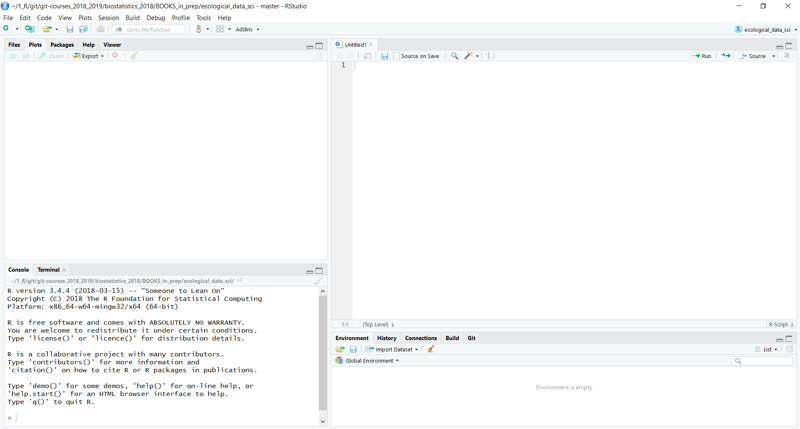
\includegraphics[width=11.11in]{/Users/nlb24/OneDrive - University of Pittsburgh/compbio4all_book/compbio4all-book/images/RStudio_1st_view-800x600} \caption{RStudio when first opened.}(\#fig:rstudio.open)
\end{figure}

When referring to RStudio (and equivalently RSTudio Cloud - this is the last time I'll mention this so hopefully get get the point), there are two terms that need to be understood. As shown in Figure 3, there is 1)the \textbf{console} section of RStudio and 2) the \textbf{script editor} or \textbf{source viewer}.

\begin{figure}
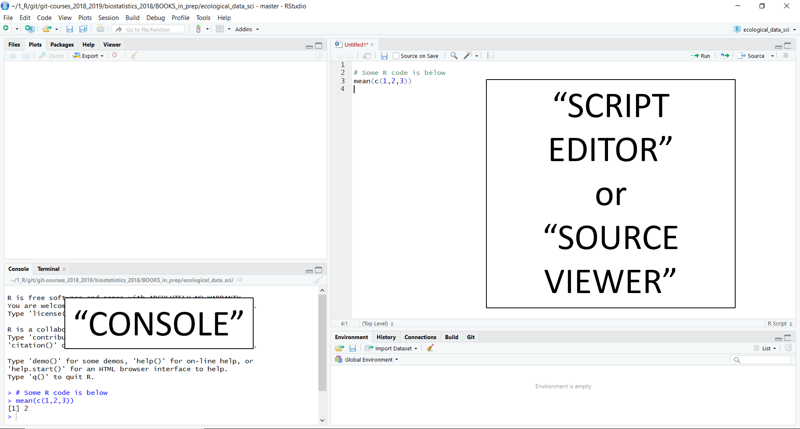
\includegraphics[width=11.11in]{/Users/nlb24/OneDrive - University of Pittsburgh/compbio4all_book/compbio4all-book/images/RStudio_console_vs_script_editor-800x600} \caption{RStudio's console and script editor.}(\#fig:rstudio.console)
\end{figure}

(A ``cheat sheet'' called the ``RStudio IDE Cheat Sheet'' details all of RStudio's many features and is available at \url{https://www.rstudio.com/resources/cheatsheets/} . It very thorough, though a bit dense. I don't recommend it for beginners but you should remember that it exists.)

\hypertarget{the-console-versus-the-script-editor}{%
\subsection{The console versus the script editor}\label{the-console-versus-the-script-editor}}

You can type and enter text into both the \textbf{console} and the \textbf{script editor} (also called the \textbf{source viewer}. The console, however, responds actively like a calculator, while the script editor works more like a text editor. Information can be passes unidirectionally from the script editor to the console, but not the other way.

\hypertarget{the-r-console}{%
\subsubsection{The R console}\label{the-r-console}}

The \textbf{console} in RStudio gives you \textbf{interactive programming} environment that is very similar to a scientific calculator. If you click your mouse inside the console and type \texttt{1\ +\ 1} then press enter you will see the following type of output

\begin{Shaded}
\begin{Highlighting}[]
\DecValTok{1} \SpecialCharTok{+} \DecValTok{1}
\end{Highlighting}
\end{Shaded}

\begin{verbatim}
## [1] 2
\end{verbatim}

Note that right in front of where you typed \texttt{1+1} there is a \texttt{\textgreater{}} symbol. This is always in the R console and never needs to be typed. You may occasionally see it printed in books or on websites, but it doesn't ever need to be typed.

One thing to note about R is that it's not particular about spacing. All of the following things will yield the same results

\begin{Shaded}
\begin{Highlighting}[]
\DecValTok{1}\SpecialCharTok{+}\DecValTok{1}
\DecValTok{1} \SpecialCharTok{+} \DecValTok{1}
\DecValTok{1}          \SpecialCharTok{+}        \DecValTok{1}
\DecValTok{1} \SpecialCharTok{+}                                   \DecValTok{1}
\end{Highlighting}
\end{Shaded}

Got it? Awesome! Now we're ready for some real data analysis.

  \bibliography{book.bib,packages.bib}

\end{document}
